
\chapter{Referencias al proyecto}

\section{Referencias en blogs}

El modelo de desarrollo abierto y colaborativo del proyecto ha conseguido que el proyecto
haya entrado de manera natural en la comunidad científica que trabaja en el campo de la
Web Semántica.

Esto ha hecho que dicha comunidad haya seguido con interés los avances en el proyecto,
coleccionando un puñado de citas que siempre son de agradecer:

\subsection*{SIOC News\footnote{\url{http://apassant.net/blog/post/2006/10/01/117-sioc-news}}}

Por Alexandre Passant el domingo 1 de Octubre de 2006, día previo al lanzamiento 
de la primera versión de SWAML:

\begin{quote}
 (...) Wikier mentionned on \#sioc that SWAML, a project he's involved in to translate mailing 
 lists in RDF, will use SIOC. (...)
\end{quote}

\subsection*{State of the SIOC-o-sphere\footnote{\url{http://www.johnbreslin.com/blog/2006/11/07/state-of-the-sioc-o-sphere-number-3/}}}

Por John Breslin el martes 7 de Noviembre de 2006, después de la publicación de Buxon:

\begin{quote}
 (...) SWAML, the Semantic Web Archive of Mailing Lists, is now using SIOC as its base 
 ontology. Last week, the developers also announced that SWAML now incorporates Buxon, a sioc:Forum 
 visor written in PyGTK (see screenshot). Excellent stuff  (...)
\end{quote}

\subsection*{Buxon visor for sioc:Forum browsing\footnote{\url{http://www.johnbreslin.com/blog/2006/11/08/buxon-visor-for-siocforum-browsing/}}}

Por John Breslin el miércoles 8 de Noviembre de 2006, dando su impresión de Buxon:

\begin{quote}
 I've been testing out the Buxon visor for browsing SIOC forums, created by the SWAML 
 developers and written in PyGTK.

 So far, it works great (with SWAML-generated data). I used an example script packaged 
 with python-libgmail (archive.py) to download an inbox from a GMail account (subscribed 
 to the sioc-dev mailing list) to mbox format, and then ran swaml.py on that mbox to 
 convert it to SIOC RDF. The resulting RDF is here, and I successfully browsed this with 
 Buxon. Great job, SWAML guys!

 This is a nice demonstrator, and it just remains to do the same for a few more 
 SW-related mailing lists...
\end{quote}

\section{Otras referencias}

\subsubsection*{nice phone from Patrick\footnote{\url{http://flickr.com/photos/leobard/294518500/in/pool-iswc/}}}

Uldis Bojars comendo en la lista de correo de SIOC-Dev\footnote{\url{http://groups.google.com/group/sioc-dev/browse_thread/thread/c9689c4762390396/674fa1a9fedfc1ac}}
la foto que había hecho en el ISWC2006\footnote{\url{http://iswc2006.semanticweb.org/}}
con PlanetRDF\footnote{\url{http://planetrdf.com/}} visto desde un móvil. Con la casualidad
que el post que en ese momento estaba en portada era el de John Breslin hablando de Buxon,
como se puede ver en la figura~\ref{fig:planetrdf-mobile}.

\begin{figure}[ht]
	\centering
	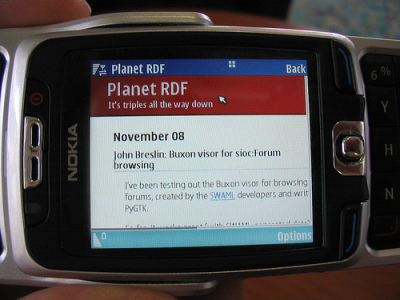
\includegraphics{images/screenshots/planetrdf-mobile.png}
	\caption{PlanetRDF visto desde un móvil con un post hablando de Buxon}
	\label{fig:planetrdf-mobile}
\end{figure}


